\chapter{Онолын хэсэг}
\section{Өнөөгийн байдлын судалгаа}

Судалгааны хүрээнд Монгол Улсад сувилал, амралтын газрын үйлчилгээтэй холбоотой цахим шийдлүүдийг харьцуулан судлав. Үүнд Шаргалжуут сувиллын веб сайт, Zugaalga.mn, Baatarvan.com болон iHotel.mn платформуудыг сонгон шинжилсэн. Эдгээр системүүдийн онцлогийг Хүснэгт~\ref{tab:similar-systems}-д нэгтгэн үзүүлэв.

\begin{table}[H]
  \centering
  \caption{Ижил төстэй системүүдийн харьцуулалт}
  \label{tab:similar-systems}
  \renewcommand{\arraystretch}{1.3}
  \begin{tabular}{p{4cm}p{9cm}}
    \toprule
    \textbf{Систем} & \textbf{Онцлог} \\
    \midrule
    Шаргалжуут сувиллын веб сайт &
    Байгууллагын мэдээлэл түгээх зориулалттай статик веб сайт бөгөөд захиалгын үйл ажиллагааг бүрэн цахимжуулаагүй. \\
    \hline
    Zugaalga.mn &
    Амралт, аялал жуулчлалын байгууллагуудын мэдээллийн нэгдсэн сан боловч хэрэглэгч шууд захиалга хийх боломжгүй. \\
    \hline
    Baatarvan.com &
    Үйлчилгээний танилцуулга болон мэдээлэл агуулдаг боловч онлайн захиалга хийдэггүй. \\
    \hline
    iHotel.mn &
    Зочид буудал, амралтын газрын захиалгын платформ боловч сувиллын үйлчилгээний онцлогийг хангаагүй. \\
    \bottomrule
  \end{tabular}
\end{table}

Шаргалжуут сувиллын албан ёсны веб сайт нь байгууллагын танилцуулга, үйлчилгээний мэдээлэл хүргэх зориулалттай статик бүтэцтэй бөгөөд захиалгын үйл ажиллагааг Google Form ашиглан шийдсэн байсан \cite{shargaljuut2026}. Zugaalga.mn нь амралт, аялал жуулчлалын үйлчилгээний нэгдсэн мэдээллийн сан хэлбэрээр ажилладаг боловч хэрэглэгч шууд өрөө захиалах боломжгүй \cite{zugaalga2026}. Baatarvan.com нь байгууллагын мэдээлэл болон үйлчилгээний танилцуулга агуулсан хэдий ч захиалга удирдах функцгүй байна \cite{baatarvan2026}. Харин iHotel.mn нь зочид буудал, амралтын газрын онлайн захиалгын систем боловч сувиллын байгууллагын эмчилгээний багц, хэвтэн эмчлүүлэх хугацаа зэрэг онцлог шаардлагыг дэмждэггүй \cite{ihotel2026}.

Хүснэгт~\ref{tab:similar-systems}-ээс харахад судалсан системүүдийн аль нь ч сувиллын байгууллагын өрөөний захиалга, эмчилгээний багц болон хэрэглэгчийн мэдээллийг нэгдсэн байдлаар удирдах боломжийг бүрэн хангаагүй байна. Иймээс сувиллын үйлчилгээний онцлогт нийцсэн, захиалга болон мэдээллийн удирдлагыг нэгтгэсэн веб систем боловсруулах шаардлага байгааг энэхүү судалгаа харуулж байна.

\section{Захиалгын системийн тухай ойлголт}

Онлайн захиалгын систем гэдэг нь хэрэглэгчдэд интернэтийн сүлжээгээр дамжуулан үйлчилгээ захиалах боломж олгодог программ хангамжийн шийдэл юм. Уг систем нь уламжлалт утас болон биечлэн хандах захиалгын аргыг орлуулж, байгууллага болон хэрэглэгч хоёрын хоорондын харилцааг цахим орчинд шилжүүлдэг.

Онлайн захиалгын системийн үндсэн үйл ажиллагааг дараах чиглэлээр авч үзнэ:

\begin{itemize}
  \item \textbf{Хүртээмжийн шалгалт.} Хэрэглэгч тодорхой огноо, хугацаанд боломжит үйлчилгээ буюу өрөөний мэдээллийг цаг тухайд нь харах боломжтой.
  \item \textbf{Захиалга бүртгэл.} Хэрэглэгч өөрийн хувийн мэдээлэл, сонгосон үйлчилгээний мэдээллийг оруулж захиалга үүсгэнэ.
  \item \textbf{Баталгаажуулалт ба мэдэгдэл.} Ажилтан захиалгыг хянаж баталгаажуулах бөгөөд системд бүртгэгдсэн хэрэглэгчид мэдэгдэл хүргэнэ.
  \item \textbf{Захиалга удирдлага.} Хэрэглэгч болон ажилтан захиалгын төлөвийг хянах, өөрчлөх, цуцлах боломжтой.
  \item \textbf{Тайлан, статистик.} Байгууллага захиалгын мэдээлэлд тулгуурлан гүйцэтгэлийн тайлан гаргана.
\end{itemize}

Байгууллагад онлайн захиалгын системийг нэвтрүүлснээр хэд хэдэн давуу тал бий болдог. Нэгдүгээрт, цахим системийн тусламжтайгаар хэрэглэгч өдрийн аль ч цагт, хаана ч байсан захиалга хийх боломжтой болох тул байгууллагын үйлчилгээний хүртээмж мэдэгдэхүйц нэмэгддэг. Хоёрдугаарт, утасны харилцаа болон гараар бүртгэх ажиллагааг автоматжуулснаар ажилтнуудын цагийг хэмнэж, алдааны эрсдэлийг багасгадаг. Гуравдугаарт, захиалгын бүх мэдээлэл өгөгдлийн санд бүртгэгдэж хадгалагддаг тул дараагийн шийдвэр гаргалтад ашиглах боломжтой мэдээллийн эх сурвалж бүрддэг.

% ─────────────────────────────────────────────────────────────
\section{Веб мэдээллийн системийн үндсэн ойлголт}

\subsection{Client--Server загвар}

Client--Server загвар нь орчин үеийн веб системийн суурь архитектурын зарчим юм \cite{tanenbaum2007}. Энэхүү загварт хоёр талын оролцогч байдаг: хэрэглэгчийн хүсэлт илгээдэг клиент (client) болон тухайн хүсэлтийг боловсруулж хариу буцаадаг сервер (server).

\begin{figure}[H]
  \centering
  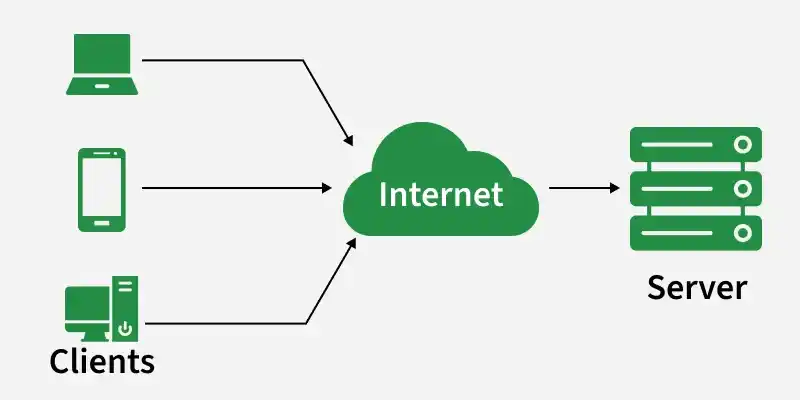
\includegraphics[width=0.75\textwidth]{figures/client-server.png}
  \caption{Client--Server загварын харилцан үйлчлэл}
  \label{fig:client-server}
\end{figure}
Веб системд хэрэглэгчийн хөтөч нь клиентийн үүрэг гүйцэтгэж, сервертэй HTTP хүсэлт болон хариугаар харилцдаг. Хэрэглэгчийн илгээсэн хүсэлтийг сервер боловсруулж, шаардлагатай өгөгдөл эсвэл хуудсыг буцаан илгээдэг. Ийнхүү клиент болон серверийн үүргийг тусгаарласнаар системийг хөгжүүлэх, засварлах болон өргөтгөх боломж сайжирдаг.

\subsection{REST API зарчим}

REST (Representational State Transfer) нь веб системийн програмчлалын интерфейсийн архитектурын хэв загвар бөгөөд Fielding \cite{fielding2000} анх тодорхойлсон. REST зарчимд суурилсан интерфейсийг RESTful API гэж нэрлэх бөгөөд орчин үеийн веб системүүд хоорондын өгөгдөл солилцооны гол арга хэлбэр болж байна.

RESTful API нь нөөц бүрийг URL хаягаар тодорхойлж, тухайн нөөцтэй хийх үйлдлийг HTTP арга (GET, POST, PUT, DELETE)-аар илэрхийлдэг. Жишээлбэл, энэхүү судалгааны ажлын системд амрагч шинэ захиалга үүсгэхдээ \texttt{POST /api/bookings} хүсэлтийг серверт илгээдэг. Сервер уг хүсэлтийг боловсруулж, захиалгын дугаар болон төлвийн мэдээллийг JSON форматаар буцаана. Зураг~\ref{fig:rest-api}-д энэхүү хүсэлт-хариуны урсгалыг харуулав.

\begin{figure}[H]
  \centering
  \begin{tikzpicture}[
    node distance=0.55cm,
    client/.style={rectangle, draw=gray!60, fill=gray!10, rounded corners=4pt,
                   minimum width=5.5cm, minimum height=0.75cm,
                   align=center, font=\small\bfseries},
    payload/.style={rectangle, draw=blue!40, fill=blue!6, rounded corners=3pt,
                    minimum width=5.5cm, align=left,
                    font=\ttfamily\scriptsize, inner sep=7pt},
    server/.style={rectangle, draw=orange!60, fill=orange!12, rounded corners=4pt,
                   minimum width=5.5cm, minimum height=0.75cm,
                   align=center, font=\small\bfseries},
    response/.style={rectangle, draw=teal!50, fill=teal!7, rounded corners=3pt,
                     minimum width=5.5cm, align=left,
                     font=\ttfamily\scriptsize, inner sep=7pt},
    arr/.style={-{Latex[length=2.8mm,width=2mm]}, thick}
  ]
    \node[client]  (cli)  {Хэрэглэгч (хөтөч)};

    \node[payload, below=of cli] (req)
      {POST /api/bookings\\[2pt]
       \{"roomId": 5,\\
       \ "checkIn": "2026-07-01"\}};

    \node[server, below=of req]  (srv)  {Сервер};

    \node[response, below=of srv] (res)
      {HTTP/1.1\ \ 201 Created\\[2pt]
       \{"bookingId": 101,\\
       \ "status": "PENDING"\}};

    \node[client, below=of res] (cli2) {Хэрэглэгч (хариу хүлээн авна)};

    \draw[arr, blue!55]  (cli)  -- node[right, font=\scriptsize\itshape, text=blue!70]{HTTP хүсэлт} (req);
    \draw[arr, blue!55]  (req)  -- (srv);
    \draw[arr, teal!65]  (srv)  -- node[right, font=\scriptsize\itshape, text=teal!70]{HTTP хариу} (res);
    \draw[arr, teal!65]  (res)  -- (cli2);
  \end{tikzpicture}
  \caption{REST API-ийн хүсэлт болон хариуны жишээ}
  \label{fig:rest-api}
\end{figure}

REST API-ийн үндсэн онцлог нь төлөвгүй байдал буюу statelessness юм — сервер клиентийн өмнөх хүсэлтийн мэдээллийг хадгалдаггүй бөгөөд хүсэлт бүр бие даасан, бүрэн мэдээлэл агуулсан байна. Энэхүү зарчим нь клиент болон серверийн хөгжүүлэлтийг бие биенээсээ хамааралгүй явуулах, системийг өргөтгөх боломжийг нэмэгдүүлдэг.

\subsection{Харилцаат өгөгдлийн сангийн загвар}

Харилцаат өгөгдлийн сангийн загвар (relational database model) нь өгөгдлийг хүснэгт хэлбэрээр зохион байгуулж, хүснэгтүүдийн хоорондын харилцааг тодорхойлсон загвар юм \cite{elmasri2015}. Хүснэгт бүр мөр болон баганаас бүрдэнэ.

Загварын гол ойлголтууд:

\begin{itemize}
  \item \textbf{Анхдагч түлхүүр (Primary Key).} Хүснэгтийн мөр бүрийг давтагдашгүй байдлаар таньж тодорхойлдог талбар. Ихэвчлэн автоматаар үүсдэг тоон утга ашигладаг.
  \item \textbf{Гадаад түлхүүр (Foreign Key).} Нэг хүснэгтийн мөрийг өөр хүснэгтийн мөртэй холбох талбар. Хүснэгтүүдийн хоорондын харилцааг тодорхойлно.
  \item \textbf{Нэг-олон харилцаа (One-to-Many).} Нэг хүснэгтийн нэг мөр өөр хүснэгтийн олон мөртэй харилцаатай байх тохиолдол. Жишээ нь нэг амрагч олон захиалга үүсгэж болно.
\end{itemize}

Хүснэгтүүд болон тэдгээрийн хоорондын харилцааг дүрслэхэд Entity-Relationship диаграмм ашигладаг. Зураг~\ref{fig:er-theory}-д хоёр хүснэгтийн хоорондох нэг-олон харилцааны энгийн жишээг үзүүлэв.

\begin{figure}[H]
  \centering
  \begin{tikzpicture}[
    tbl/.style={
      rectangle, draw, rounded corners=4pt,
      minimum width=3.8cm, align=left,
      font=\small, inner sep=8pt
    },
    hdr/.style={
      rectangle, draw, rounded corners=4pt,
      fill=gray!20, minimum width=3.8cm,
      align=center, font=\small\bfseries,
      inner sep=6pt
    },
    arr/.style={-{Latex[length=3mm]}, thick, gray!70!black}
  ]
    % Хэрэглэгч хүснэгт
    \node[hdr] (u_hdr) at (0,0) {Хэрэглэгч};
    \node[tbl, below=-\pgflinewidth of u_hdr, anchor=north] (u_body)
      {\underline{id} (PK)\\нэр\\утас\\үүрэг};

    % Захиалга хүснэгт
    \node[hdr] (b_hdr) at (6,0) {Захиалга};
    \node[tbl, below=-\pgflinewidth of b_hdr, anchor=north] (b_body)
      {\underline{id} (PK)\\хэрэглэгч\_id (FK)\\өрөө\_id\\статус};

    % Холбоос
    \draw[arr] (u_body.east) -- node[above, font=\scriptsize]{1 : N} (b_body.west);
  \end{tikzpicture}
  \caption{Хүснэгтүүдийн хоорондох нэг-олон харилцааны жишээ}
  \label{fig:er-theory}
\end{figure}

Энэхүү загварыг ашигласнаар өгөгдлийн бүрэн бүтэн байдал, давхардлаас сэргийлэх, хурдан хайлт хийх боломж бүрддэг.

\subsection{Нэвтрэлт ба баталгаажуулалтын ойлголт}

Веб системийн аюулгүй байдлын хүрээнд \textit{нэвтрэлт баталгаажуулалт} (authentication) болон \textit{эрх шалгалт} (authorization) гэсэн хоёр ялгаатай ойлголт байдаг. Зураг~\ref{fig:auth-theory}-д эдгээр хоёр ойлголтын ялгааг харуулав.

\begin{figure}[H]
  \centering
  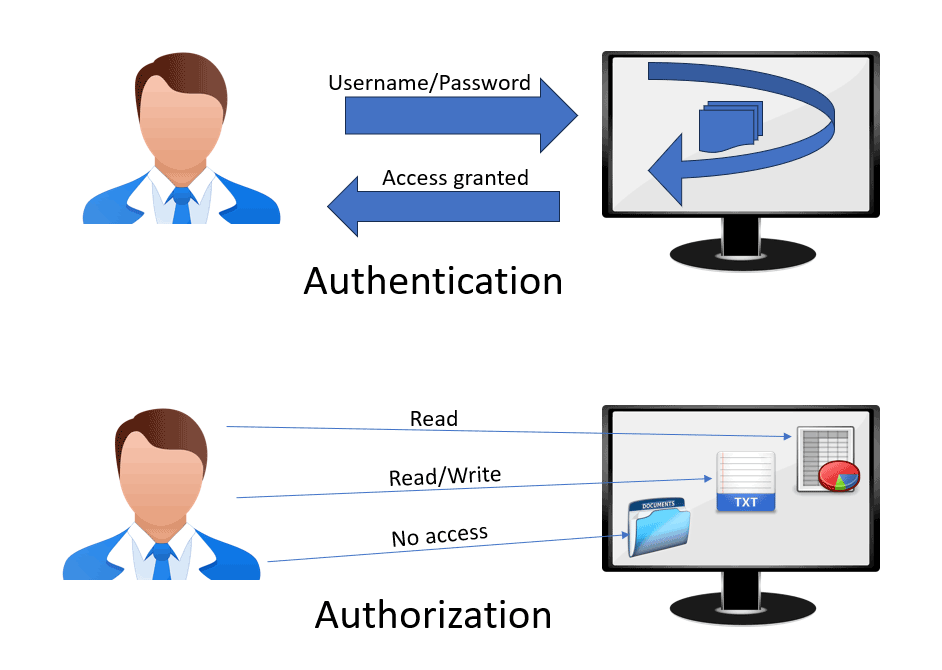
\includegraphics[width=0.72\textwidth]{figures/auth-vs-authz.png}
  \caption{Нэвтрэлт баталгаажуулалт ба эрх шалгалтын ялгаа}
  \label{fig:auth-theory}
\end{figure}

Нэвтрэлт баталгаажуулалт (authentication) нь хэрэглэгч хэн болохыг тогтоох үйл явц бөгөөд эрх шалгалт (authorization) нь тухайн хэрэглэгч системийн ямар нөөцөд хандах боломжтойг тодорхойлдог. Жишээлбэл, зарим хэрэглэгч зөвхөн мэдээлэл харах эрхтэй бол админ хэрэглэгч нэмэх, засах, устгах зэрэг нэмэлт эрхтэй байж болно.

Токенд суурилсан баталгаажуулалтын хүрээнд JSON Web Token (JWT) нь өргөн хэрэглэгддэг стандарт бөгөөд IETF-ийн RFC~7519-ээр тодорхойлогдсон \cite{jones2015jwt}. JWT нь хэрэглэгчийн мэдээллийг агуулсан токен ашиглан серверт сейшн хадгалахгүйгээр хэрэглэгчийг таних боломж олгодог. Энэхүү системд JWT-д суурилсан нэвтрэлт болон эрхийн хяналтыг ашиглаж, хэрэглэгчийг амрагч болон админ гэсэн хоёр үүргээр ялган хэрэгжүүлсэн.